\section{Задание 3. Аппроксимация константной моделью}

\subsection{Постановка задачи}

Для данных варианта 11 (см. таблицу~\ref{tab:data}) найти наилучшую аппроксимацию константной моделью $z(x, y) \equiv c$:
\begin{enumerate}
    \item в смысле минимизации MSE (среднеквадратичной ошибки);
    \item в смысле минимизации MAE (средней абсолютной ошибки).
\end{enumerate}

\subsection{Теоретическое обоснование}

\textbf{Минимизация MSE.} Функция потерь:
\begin{equation}
    L_{\text{MSE}}(c) = \frac{1}{N}\sum_{i=1}^{N}(c - z_i)^2.
\end{equation}
Приравнивая производную к нулю: $\frac{dL}{dc} = \frac{2}{N}\sum(c - z_i) = 0$, получаем:
\begin{equation}
    c_{\text{MSE}} = \frac{1}{N}\sum_{i=1}^{N} z_i = \overline{z}.
\end{equation}
Оптимальной константой в смысле MSE является \textbf{среднее арифметическое} значений $z$. Это является следствием того, что минимизация MSE эквивалентна максимизации функции правдоподобия в предположении нормального распределения ошибок.

\textbf{Минимизация MAE.} Функция потерь:
\begin{equation}
    L_{\text{MAE}}(c) = \frac{1}{N}\sum_{i=1}^{N}|c - z_i|.
\end{equation}
Субградиент: $\frac{\partial L}{\partial c} = \frac{1}{N}\sum \text{sign}(c - z_i)$. Минимум достигается когда $c$ равно \textbf{медиане} выборки $\{z_i\}$:
\begin{equation}
    c_{\text{MAE}} = \text{median}(z_1, \ldots, z_N).
\end{equation}
Минимизация MAE эквивалентна максимизации функции правдоподобия в предположении распределения Лапласа ошибок.

\subsection{Результаты}

Для варианта 11 значения $z$: $\{0.73, 3.65, 4.86, 2.00, 0.32\}$.

\begin{itemize}
    \item Упорядоченные значения: $0.32, 0.73, 2.00, 3.65, 4.86$.
    \item Среднее арифметическое: $\overline{z} = \frac{0.73 + 3.65 + 4.86 + 2.00 + 0.32}{5} = 2.3120$.
    \item Медиана: $\text{median}(z) = 2.00$ (третий элемент в упорядоченной выборке из 5 значений).
\end{itemize}

\begin{table}[H]
    \centering
    \caption{Результаты аппроксимации константной моделью}
    \label{tab:const_results}
    \begin{tabular}{|l|c|c|c|c|}
        \hline
        \textbf{Критерий} & \textbf{Константа $c$} & \textbf{Метод} & \textbf{MSE} & \textbf{MAE} \\
        \hline
        MSE & 2.3120 & Среднее арифм. & 2.9701 & 1.5544 \\
        MAE & 2.0000 & Медиана & 3.0675 & 1.4920 \\
        \hline
    \end{tabular}
\end{table}

\subsection{Таблицы невязок}

\begin{table}[H]
    \centering
    \caption{Невязки MSE-оптимальной константы ($c = \overline{z} = 2.3120$)}
    \label{tab:const_mse}
    \begin{tabular}{|c|c|c|c|c|c|}
        \hline
        \textbf{Точка} & \textbf{$x$} & \textbf{$y$} & \textbf{$z_{факт}$} & \textbf{$z_{модель}$} & \textbf{Невязка} & \textbf{Кв. невязки} \\
        \hline
        0 & 0.85 & 1.12 & 0.73 & 2.3120 & 1.5820 & 2.5027 \\
        1 & 1.83 & 2.20 & 3.65 & 2.3120 & -1.3380 & 1.7902 \\
        2 & 2.91 & 3.12 & 4.86 & 2.3120 & -2.5480 & 6.4923 \\
        3 & 3.93 & 3.92 & 2.00 & 2.3120 & 0.3120 & 0.0973 \\
        4 & 4.86 & 4.94 & 0.32 & 2.3120 & 1.9920 & 3.9681 \\
        \hline
    \end{tabular}
\end{table}

\begin{table}[H]
    \centering
    \caption{Невязки MAE-оптимальной константы ($c = \text{median}(z) = 2.0000$)}
    \label{tab:const_mae}
    \begin{tabular}{|c|c|c|c|c|c|}
        \hline
        \textbf{Точка} & \textbf{$x$} & \textbf{$y$} & \textbf{$z_{факт}$} & \textbf{$z_{модель}$} & \textbf{Невязка} & \textbf{|Невязка|} \\
        \hline
        0 & 0.85 & 1.12 & 0.73 & 2.0000 & 1.2700 & 1.2700 \\
        1 & 1.83 & 2.20 & 3.65 & 2.0000 & -1.6500 & 1.6500 \\
        2 & 2.91 & 3.12 & 4.86 & 2.0000 & -2.8600 & 2.8600 \\
        3 & 3.93 & 3.92 & 2.00 & 2.0000 & 0.0000 & 0.0000 \\
        4 & 4.86 & 4.94 & 0.32 & 2.0000 & 1.6800 & 1.6800 \\
        \hline
    \end{tabular}
\end{table}

\subsection{Визуализация}

\begin{figure}[H]
    \centering
    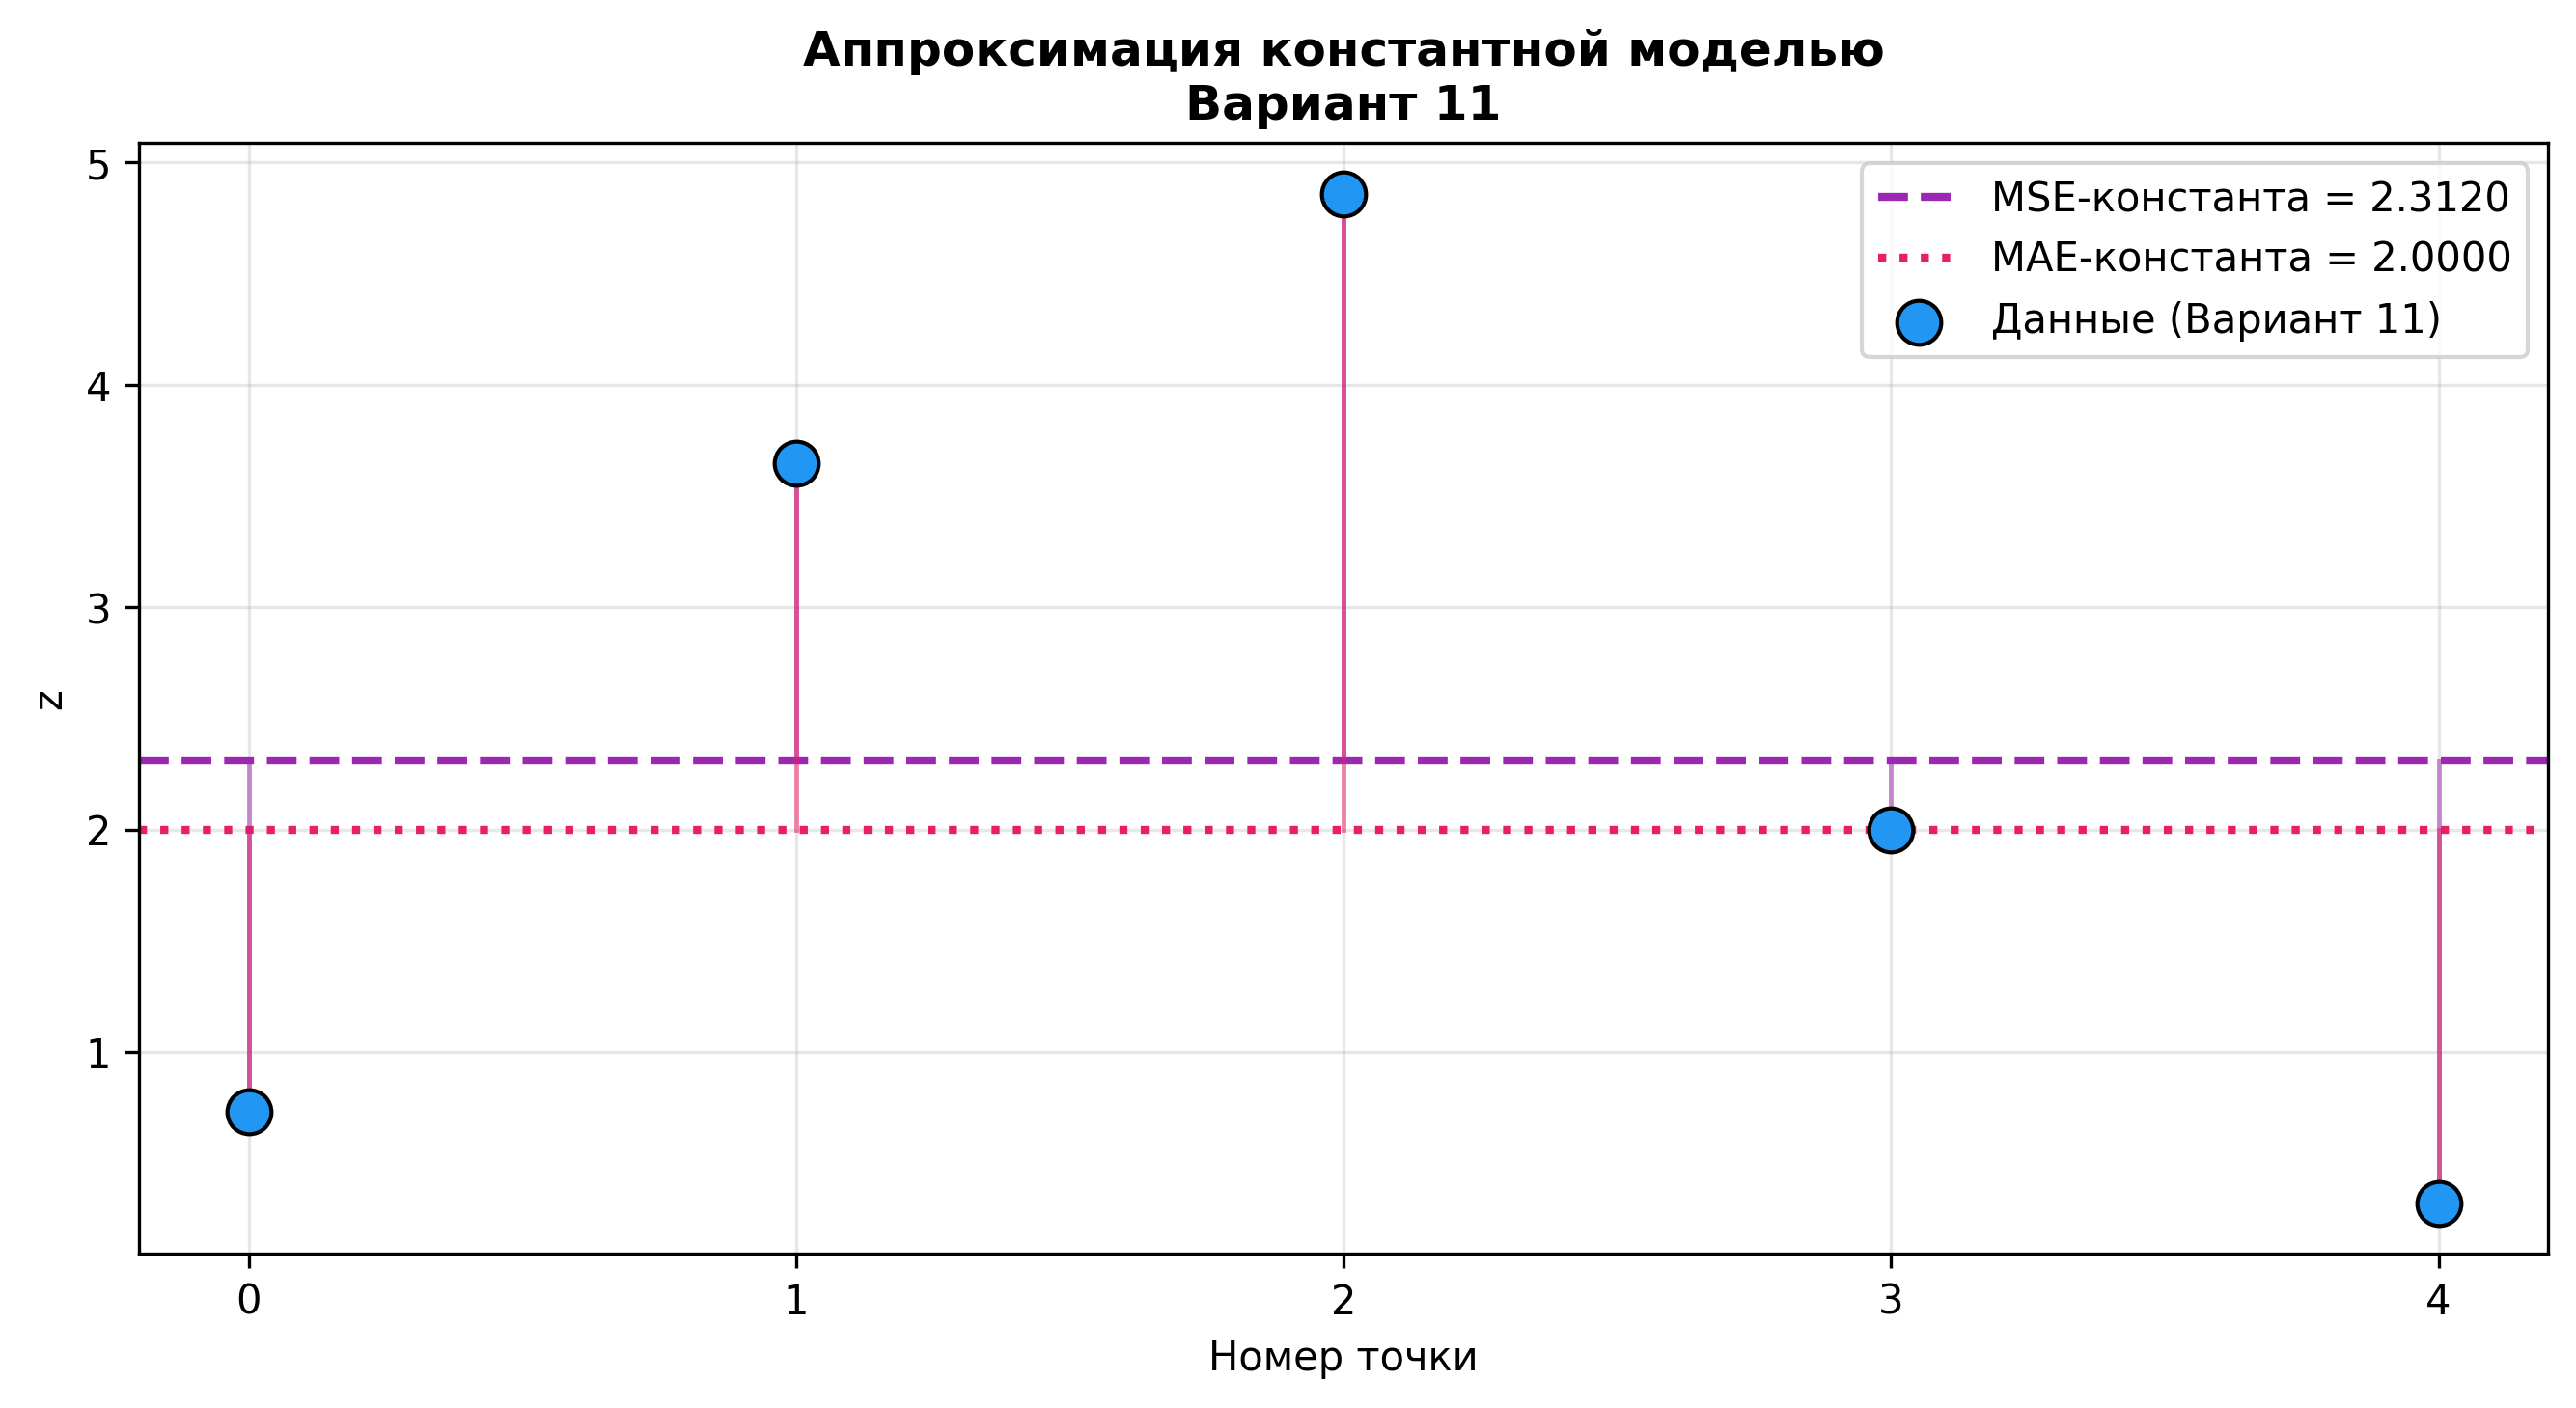
\includegraphics[width=0.85\textwidth]{pic/constant_model.png}
    \caption{Аппроксимация константной моделью (Вариант 11)}
    \label{fig:const_model}
\end{figure}

На рис.~\ref{fig:const_model} показаны две константы: $c_{\text{MSE}} = 2.3120$ (среднее) и $c_{\text{MAE}} = 2.0000$ (медиана). Видно, что MAE-константа проходит через точку 3 (значение которой совпадает с медианой), а MSE-константа даёт компромиссное значение, штрафуя большие отклонения квадратично.

\subsection{Вывод}

Константная модель имеет только один параметр и даёт $\text{MSE} = 2.97$ (для $c_{\text{MSE}}$) или $\text{MAE} = 1.49$ (для $c_{\text{MAE}}$). Эти ошибки значительно превосходят ошибки гауссианы и RBF-сети. Константная модель является простейшим базовым уровнем (baseline), относительно которого оценивается качество более сложных моделей: гауссиана уменьшает MSE в $\sim 10^{10}$ раз, что демонстрирует её высокую эффективность для данных колоколообразной формы.
